\documentclass[10pt,a4paper]{article}
\usepackage[T1]{fontenc}
\usepackage[utf8]{inputenc}
\usepackage[margin=22mm]{geometry}
\usepackage{lmodern,microtype,amsmath,amssymb,booktabs,tabularx,graphicx,float,xcolor}
\usepackage[font=small,labelfont=bf]{caption}
\usepackage[colorlinks=true,linkcolor=blue,citecolor=blue,urlcolor=blue]{hyperref}
\usepackage{url}
\graphicspath{{figures/}}
\setlength{\parskip}{4pt}
\setlength{\parindent}{0pt}
\emergencystretch=2em
\newcommand{\CO}{CO\textsubscript{2}}
\title{Regime-Dependent Routing-Policy Preference:\\When Adapting an Established Routing Policy Pays, and When It Does Not}
\author{Author details to be supplied}
\date{Conference submission draft --- 21 September 2026}
\begin{document}
\maketitle

\begin{abstract}
Navigation systems implement several established pre-trip routing objectives --- shortest distance, dynamic travel time, constrained eco-routing --- but the choice \emph{among} them is normally fixed by design rather than by traffic condition. We characterise that choice empirically. In 432 completed SUMO simulations over 24 controlled contexts on a 12-signal urban mesh, the preferred policy reverses with demand: shortest-distance routing is preferred in every low-demand context, dynamic travel-time routing in every high-demand context, and the reversal is displaced by the signal regime, crossing between 720 and 1200\,veh/h under balanced signals but only between 1200 and 1680\,veh/h under arterial-priority signals. The reversal is worth having: adapting the policy rather than fixing it removes 0.03018 units of mean decision regret against the best fixed policy, and a depth-3 regression tree predicting policy outcomes from pre-decision context recovers 79.9\% of that headroom under leave-one-context-out evaluation (mean regret 0.00606, 21/24 contexts optimal). The same selector is \emph{harmful} when the held-out context lies outside the demand range it was trained on: holding out an entire demand level, mean regret rises to 0.07649 against 0.03018 for the best fixed policy. Two audited negative controls bound the scope: an environmental routing objective collapsed onto shortest-distance routing (outcome-identical in 21/24 contexts; 21.62\% route-order selection loss) and was removed from the portfolio, and the preference weights left every selector decision unchanged across the full time-to-emissions range. Adaptive routing-policy selection is therefore governed by regime coverage of the context space, not by model capacity. We introduce no routing, decision or learning algorithm.
\end{abstract}
\textbf{Keywords:} routing-policy selection; traffic regimes; SUMO; decision regret; algorithm selection; eco-routing.

\section{Introduction}
Choosing a route and choosing a \emph{routing policy} are different decisions. A pre-trip planner may minimise distance, estimated travel time, or an estimated environmental cost; production navigation systems commit to one such objective and apply it uniformly. Whether that commitment costs anything, and under what conditions, is an empirical question about the traffic environment rather than about the planner.

This paper answers it for a controlled synthetic environment. Our question is:
\begin{quote}
\emph{Under what traffic regimes does the preferred routing policy change, how much decision value is available from adapting that policy, and how reliably can the resulting structure be identified on unseen and out-of-regime contexts?}
\end{quote}

The object of study is the mapping from observable pre-trip context to preferred established policy. A learned selector appears only as the instrument that tests whether that mapping is recoverable; it is not the contribution. We report four findings, each from completed simulation evidence.

\textbf{(1) Routing-policy preference is regime-structured.} Shortest-distance routing (SP) is preferred in all eight low-demand contexts and dynamic travel-time routing (DTT) in all eight high-demand contexts. The preference reverses monotonically in demand in every one of the eight restriction/signal cells.

\textbf{(2) The signal regime displaces the reversal.} Under balanced signal timing the reversal occurs between 720 and 1200\,veh/h in all four restriction configurations; under arterial-priority timing it occurs between 1200 and 1680\,veh/h in three of four. The signalisation plan, not only the demand, determines where policy adaptation begins to matter.

\textbf{(3) The headroom is real and largely recoverable.} Adapting the policy is worth 0.03018 mean additive regret units against the best fixed policy. A depth-3 regression tree recovers 79.9\% of it on held-out contexts.

\textbf{(4) There is an extrapolation boundary.} The same selector applied to an unseen demand regime is worse than simply fixing the best policy. The operative requirement is that training contexts span the regimes that will be met.

We claim no new routing algorithm, no new multi-criteria method and no new learning algorithm. Two prior negative results from the same project --- a failed environmental route-cost estimator and an inert preference layer --- are retained as audited controls that delimit what the positive findings mean.

\section{Related work}
\textbf{Routing strategies and regime effects.} That routing-strategy performance depends on network load is established. Analytical work on non-Markovian routing dynamics derives distinct efficiency phases as a function of the mix between shortest-time and shortest-distance preference, showing that routing preference can move a system between qualitatively different regimes \cite{R41}. Falek~et~al.\ ask when real-time re-routing is worthwhile and find, from three months of city speed data, that it is seldom useful except during rush hours and for long routes \cite{R42}. Novikov~et~al.\ study congestion thresholds for triggering dynamic re-routing \cite{R43}. Chen~et~al.\ evaluate a load-aware detour strategy across a range of traffic densities \cite{R44}. Du~et~al.\ report that the advantage of learning-based over rule-based re-routing is itself regime-dependent \cite{R45}.

These studies establish demand dependence for a single adaptive mechanism, typically comparing re-routing against not re-routing, and mostly on abstract or analytical models. The present study differs in object and in evaluation: the decision is a pre-trip choice \emph{among several established policies} rather than whether to re-route; it is measured in a microscopic signalised simulation; and it is scored as a decision, by regret against a hindsight benchmark on contexts withheld from fitting. We are not aware of a study that localises the demand reversal between established pre-trip policies and separately reports its signal-regime displacement; we do not claim this as a first, since our search was targeted rather than systematic.

\textbf{Established objectives.} Shortest-path optimisation provides the additive base \cite{R01}. Eco-routing from historical and real-time information, emission prediction, and travel-time-constrained eco-routing precede this work \cite{R03,R40,R04}; Huang and Peng compare shortest, fastest, eco and constrained-eco objectives with a soft time constraint \cite{R05}. The four objective types are therefore not our contribution. We implement them by enumeration over a finite legal path catalogue and disclose the hard-filter adaptation of the constrained variant.

\textbf{Algorithm selection and decision evaluation.} Rice's formulation and its modern instantiations map instance features to algorithm performance \cite{R08,R09,R10}. Xie~et~al.\ already compare route-choice models in SUMO and discuss automatic selection \cite{R38}, so context-aware routing-policy selection is not proposed here as a new concept. Our hindsight benchmark is the routing analogue of the Virtual Best Solver used in that literature \cite{R09}: it is computed after observing outcomes and is not deployable. Predictive accuracy and decision quality need not coincide \cite{R11}; we use that distinction for evaluation, not as a training loss.

\textbf{Preference modelling.} Additive value, TOPSIS, VIKOR and PROMETHEE are established \cite{R15,R12,R13,R14}. We use a fixed-reference additive cost solely to define ``preferred'' precisely, and report below that in this environment the preference weights are nearly inert --- which is a result about the environment, not an endorsement of the method.

\section{Method}
\subsection{Network, contexts and policies}
The network is a bidirectional $3\times4$ signalised mesh with 12 signalised junctions, 47 external links and 29 legal simple primary paths (Figure~\ref{fig:network}). Horizontal and vertical spacing are 400 and 300\,m. Upper, central and lower corridors carry 40, 50 and 60\,km/h limits with 1, 1 and 2 lanes; three alternative eastbound locations contain 150\,m speed-restriction segments. Signal cycles are 60\,s with EW/NS green pairs of 26/26\,s (\emph{balanced}) or 36/16\,s (\emph{arterial}), plus common clearance intervals. Lane counts are specified inputs, not calibrated capacities.

\begin{figure}[htbp]\centering
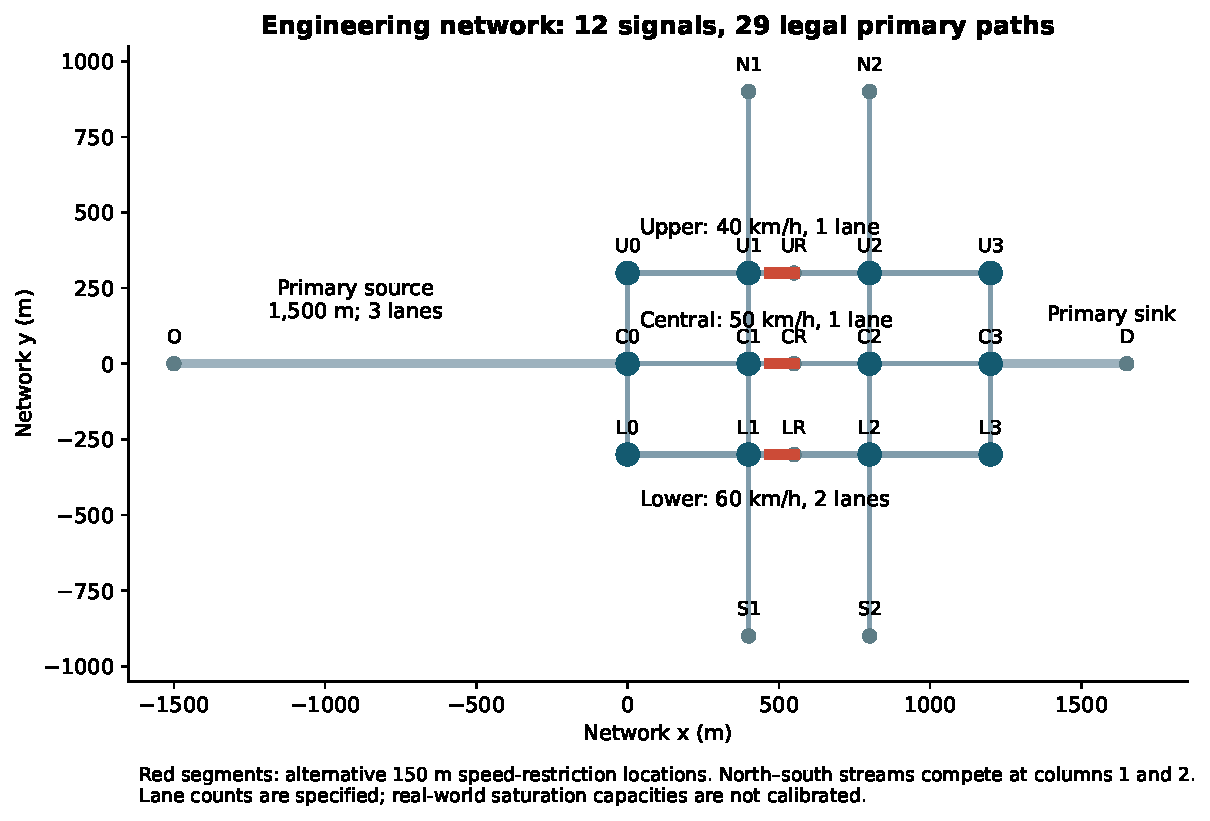
\includegraphics[width=.92\linewidth]{network.pdf}
\caption{Development network. Alternative restriction sites and competing background streams permit interacting route mechanisms.}\label{fig:network}
\end{figure}

The 24 contexts are the full factorial of primary demand $\{720,1200,1680\}$\,veh/h, restriction location $\{$none, upper, central, lower$\}$ at speed ratio 0.35, and the two signal regimes. Four background streams carry 200\,veh/h each. Each context was run under six policy settings with paired seeds 8101--8103, giving 432 completed runs. SUMO 1.25.0 was used with 1\,s steps and a homogeneous HBEFA3/PC\_G\_EU4 fleet; warm-up is 600\,s, requests stop at 2400\,s, restrictions act over 600--1200\,s, teleports are disabled. All 432 runs completed with no missing vehicles, collisions or teleports.

Let $\mathcal P$ be the 29 legal paths and $L(p)$, $\widehat T_t(p)$, $\widehat E_t(p)$ denote distance, estimated in-network time and estimated grams of \CO. The policies are
\begin{align}
p_{\mathrm{SP}}&\in\arg\min_{p\in\mathcal P}L(p), &
p_{\mathrm{DTT}}&\in\arg\min_{p\in\mathcal P}\widehat T_t(p),\\
p_{\mathrm{ECO}}&\in\arg\min_{p\in\mathcal P}\widehat E_t(p), &
p_{\mathrm{TECO}}&\in\arg\min_{p:\widehat T_t(p)\le(1+\alpha)\min_q\widehat T_t(q)}\widehat E_t(p),
\end{align}
with $\alpha\in\{5,10,15\}\%$. These are our notation and finite-candidate implementation of established objectives \cite{R01,R03,R04,R05}; the hard TECO filter is a disclosed adaptation of Huang's soft formulation. All policies share demand, signals, fleet and path catalogue; dynamic policies refresh from completed 60\,s intervals and none reroutes en route.

\textbf{Final portfolio.} Section~\ref{sec:controls} reports that ECO is outcome-identical to SP in 21 of 24 contexts and that its estimator fails route-order validation. ECO is therefore excluded from the adaptive portfolio on evidence, leaving $\mathcal A=\{\mathrm{SP},\mathrm{DTT},\mathrm{TECO}10\}$. The excluded settings are retained as controls, not discarded.

\subsection{Criteria and the definition of ``preferred''}
The estimand is the guided primary-OD cohort requested over 600--2400\,s and followed to arrival. Journey time is duration plus insertion delay; emissions are accumulated in-network tailpipe \CO. Criterion means are averaged within run, then equally across the three replications. For criterion means $y_{sak}$, positive common references $a_k$ and weights $w_k\ge0$ summing to one,
\begin{equation}
C_{sa}(w)=\sum_k w_k\frac{y_{sak}}{a_k},\qquad
R_{sa}=C_{sa}-\min_b C_{sb},
\label{eq:cost}
\end{equation}
the first being our fixed-reference linear adaptation of additive value \cite{R15} and the second opportunity loss \cite{R24}. Lower is preferred. References are the equal mean over the $24\times3$ portfolio cells: 542.844\,s and 1263.515\,g. The primary profile is balanced, $w=(0.5,0.5)$ over time and \CO.

The \emph{hindsight best-policy benchmark} $a^{\mathrm{HB}}_s=\arg\min_a C(Y_{a,s};w)$ is computed after observing outcomes. It is a benchmark, not a deployable algorithm --- the routing counterpart of the Virtual Best Solver \cite{R09}. Available headroom against a fixed policy $a_F$ is $H_s=C_{s,a_F}-C_{s,\mathrm{HB}}$. Fuel is excluded after confirming near-proportionality to \CO\ (ratio $\approx3.135$, trip correlation $>0.999999997$) for this homogeneous fleet.

\subsection{Selector and evaluation protocol}
The selector predicts \emph{policy outcomes} from pre-decision context and then applies the same frozen preference model to the predictions; it never predicts a policy label directly, so a single fitted model serves any declared weights. Features are the scheduled primary demand, the planned restriction location and speed ratio, and the signal regime --- all known before the episode. No realised outcome enters the features.

The model is a multi-output regression tree \cite{R37} of depth 3 with minimum leaf 2, predicting training-scaled time and \CO\ for each policy. Depth 3 and leaf 8 were pre-registered for a planned 84-context training set; leaf size was rescaled to the 23-context training folds used here ($8/84\rightarrow2/23$) and no other setting was varied for the reported result. Section~\ref{sec:robust} reports the full hyperparameter sweep.

With 24 contexts, the primary protocol is leave-one-context-out (LOCO): for each context, the tree \emph{and} the reference scales $a_k$ are refit on the remaining 23, and the withheld context is scored against its observed outcomes. All three replications of a context move together. We additionally report leave-one-restriction-out, a two-fold interleaved split, and --- as a deliberate stress test --- leave-one-\emph{demand}-out, which asks the selector to extrapolate to a regime it never saw. No protocol was used to choose features, model settings, scaling or comparators.

\section{Results}
\subsection{Regime structure of policy preference}\label{sec:regime}
Define the switching margin $m_s=C_{s,\mathrm{SP}}-C_{s,\mathrm{DTT}}$; negative values mean SP is preferred. Table~\ref{tab:margin} and Figure~\ref{fig:regime}(a) show that $m_s$ is negative in all eight low-demand contexts, positive in all eight high-demand contexts, and increases monotonically with demand in every cell.

\begin{table}[htbp]\centering\small
\caption{Switching margin $m=C_{\mathrm{SP}}-C_{\mathrm{DTT}}$ in common cost units. Negative: SP preferred. The sign change is bracketed by the demand grid, not localised within it.}\label{tab:margin}
\begin{tabular}{llrrrc}\toprule
Signal & Restriction & $q=720$ & $q=1200$ & $q=1680$ & Crossing bracket (veh/h)\\\midrule
Balanced & none    & $-0.0551$ & $0.4204$ & $1.0139$ & $(720,1200]$\\
Balanced & upper   & $-0.0515$ & $0.4382$ & $0.9418$ & $(720,1200]$\\
Balanced & central & $-0.0195$ & $0.8056$ & $1.1137$ & $(720,1200]$\\
Balanced & lower   & $-0.0562$ & $0.4196$ & $1.0134$ & $(720,1200]$\\\midrule
Arterial & none    & $-0.0184$ & $-0.1269$ & $0.3249$ & $(1200,1680]$\\
Arterial & upper   & $-0.0198$ & $-0.1318$ & $0.3165$ & $(1200,1680]$\\
Arterial & central & $-0.0423$ & $0.0488$ & $0.3893$ & $(720,1200]$\\
Arterial & lower   & $-0.0110$ & $-0.0954$ & $0.2952$ & $(1200,1680]$\\
\bottomrule\end{tabular}\end{table}

The signal regime displaces the reversal. Under balanced timing every cell has already crossed by 1200\,veh/h (mean margin $+0.521$); under arterial timing three of four cells have not (mean margin $-0.076$) and cross only by 1680\,veh/h. Arterial-priority timing raises the demand at which adapting the policy begins to pay by at least one grid step. The central-restriction cell crosses earlier than its siblings under both regimes, indicating an interaction between restriction placement and the crossing point that the present grid cannot resolve further.

\begin{figure}[htbp]\centering
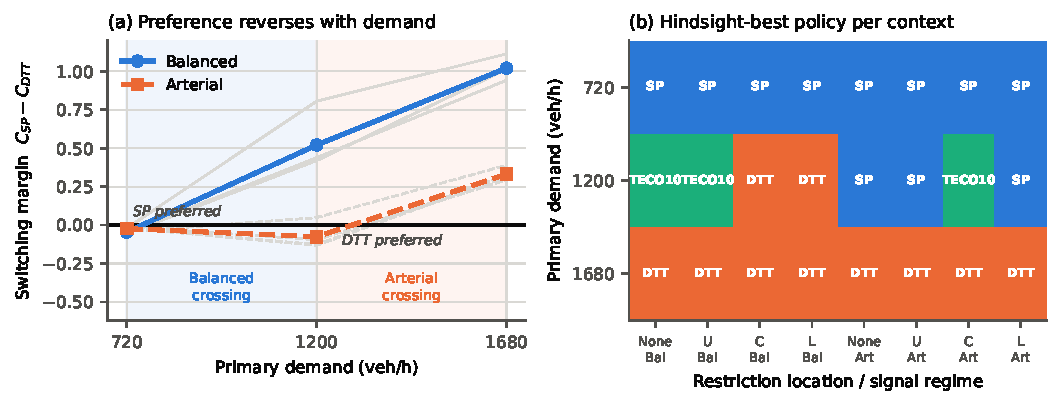
\includegraphics[width=\linewidth]{regime_structure.pdf}
\caption{(a) The switching margin reverses sign with demand; heavy lines are the mean over restriction locations, faint lines the individual cells. Shading marks the bracketing intervals, not estimated crossing points. (b) Hindsight-best policy in each of the 24 contexts.}\label{fig:regime}
\end{figure}

\textbf{Is the change abrupt or gradual?} At grid resolution the margin is monotone in demand in all eight cells and its increment grows with demand in seven of eight, i.e.\ a continuous accelerating crossing rather than a discontinuity. We emphasise what the design cannot support: with demand levels 480\,veh/h apart, the crossing is \emph{bracketed} to intervals of that width and is not localised. We therefore report brackets throughout and make no point estimate of a switching threshold. Section~\ref{sec:future} specifies the minimal experiment that would localise it.

\textbf{Cost of getting it wrong.} The penalty for a fixed policy grows sharply with demand. Mean regret of the worst available policy is 0.0342 at 720\,veh/h, 0.3229 at 1200\,veh/h and 0.6761 at 1680\,veh/h.

\textbf{Seed stability.} The hindsight-best policy is identical across all three seeds in 20 of 24 contexts, and the sign of the switching margin is stable in 22 of 24. The four unstable contexts are D005 and the three balanced-signal contexts at 1200\,veh/h --- that is, the instability sits inside the transition band, which is where ties are expected, and does not affect the low- or high-demand regimes.

\subsection{Decision headroom and held-out selection}
Fixing DTT is the best single policy but is not optimal everywhere: it leaves 0.03018 mean and 0.13176 maximum regret, and is beaten in 14 of 24 contexts. Table~\ref{tab:decision} gives the decision outcome.

\begin{table}[htbp]\centering\small
\caption{Decision quality under the balanced profile. The selector is evaluated leave-one-context-out; the hindsight benchmark is not deployable.}\label{tab:decision}
\begin{tabular}{lrrcc}\toprule
Method & Mean regret & Max regret & Optimal & Within 1\% \\\midrule
Fixed SP & 0.31825 & 1.11368 & 11/24 & 11/24 \\
Fixed DTT (best fixed) & 0.03018 & 0.13176 & 10/24 & 11/24 \\
Fixed TECO10 & 0.20757 & 1.01394 & 9/24 & 9/24 \\
\textbf{Adaptive selector (held-out)} & \textbf{0.00606} & \textbf{0.11545} & \textbf{21/24} & \textbf{22/24} \\
Hindsight best-policy benchmark & 0.00000 & 0.00000 & 24/24 & 24/24 \\
\bottomrule\end{tabular}\end{table}

The selector recovers 79.9\% of the available headroom and is optimal in 21 of 24 held-out contexts. Its out-of-sample prediction error is 44.63\,s MAE (79.73\,s RMSE) on journey time and 82.38\,g MAE (122.09\,g RMSE) on \CO, i.e.\ 8.2\% and 6.5\% of the respective means --- accurate enough to rank policies although far from exact. Leave-one-restriction-out gives the identical decision outcome; the two-fold interleaved split, with half the training data, captures 14.8\%.

All three residual errors lie in the transition band: the selector is optimal in 8/8 low-demand and 8/8 high-demand contexts, and errs only at 1200\,veh/h (D009, D011 and D014, the last contributing the 0.11545 maximum). The decision problem and the selector's difficulty occupy the same region.

\subsection{The extrapolation boundary}
Withholding an entire demand level reverses the conclusion (Figure~\ref{fig:decision}(b)). Pooled over the three folds the selector incurs 0.07649 mean regret against 0.03018 for the best fixed policy. Holding out 1680\,veh/h is the clearest failure: DTT is optimal in all eight contexts, yet the selector trained only on 720 and 1200\,veh/h chooses DTT or TECO10 and incurs 0.14856 mean regret where fixing DTT would incur none.

\begin{figure}[htbp]\centering
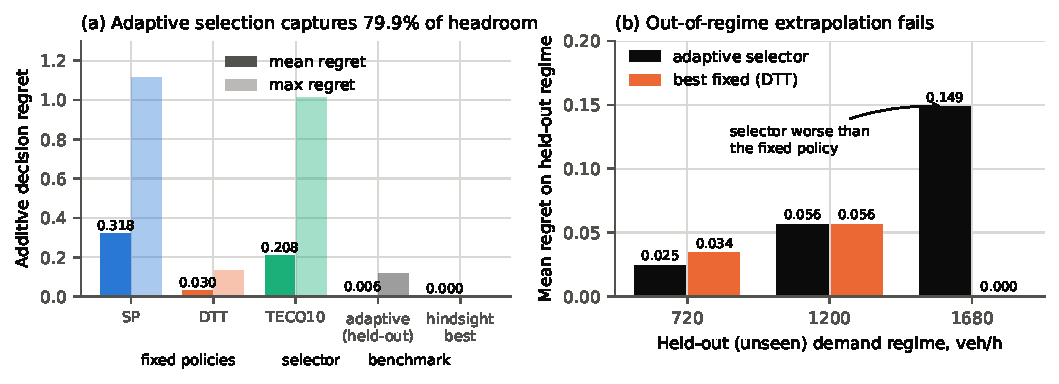
\includegraphics[width=\linewidth]{decision_outcome.pdf}
\caption{(a) Decision quality of fixed policies, the held-out selector and the hindsight benchmark. (b) Holding out an entire demand regime: the selector becomes worse than the best fixed policy.}\label{fig:decision}
\end{figure}

This is the practical boundary of the method. Within the observed regime span, interpolating between covered demand levels, adaptation is reliable and worthwhile. Outside it, a fixed policy is the safer choice. The binding requirement is coverage of the regime-defining factor rather than model capacity: a depth-1 tree already captures 53.1\% of the headroom (Section~\ref{sec:robust}).

\subsection{Negative controls}\label{sec:controls}
\textbf{The environmental objective was not a distinct policy.} ECO is outcome-identical to SP --- in time, \CO, distance and P95 to machine precision --- in 21 of 24 contexts. Its decision-time estimator passes accounting and aggregate prediction yet fails route ordering: maximum edge/trip mass discrepancy is 0.16945\% and native per-vehicle algebra error $6.945\times10^{-7}$; over 270{,}432 matched primary trips, selected-path \CO\ forecasts give WAPE 14.71\% with signed bias $-0.315\%$, improving on a frozen 600\,s snapshot (22.38\%) and a warm-up emissions-per-metre baseline (36.88\%). But in a 232-run fixed-replay probe over eight context--seed panels, in which only one tagged vehicle's route varies, the median rank correlation is 0.536 and the mean relative emission selection loss is 21.62\% against a declared 10\% screen, with a 78.16\% maximum and the predicted-best route matching the observed best in only 3 of 8 panels (Figure~\ref{fig:eco}). Good average prediction over previously selected routes did not confer correct ranking near the predicted optimum. ECO was therefore removed from the adaptive portfolio: in this environment it supplied no independent environmental decision dimension. We do not conclude that eco-routing is ineffective in general, only that this estimator in this environment did not support a distinct policy.

\begin{figure}[htbp]\centering
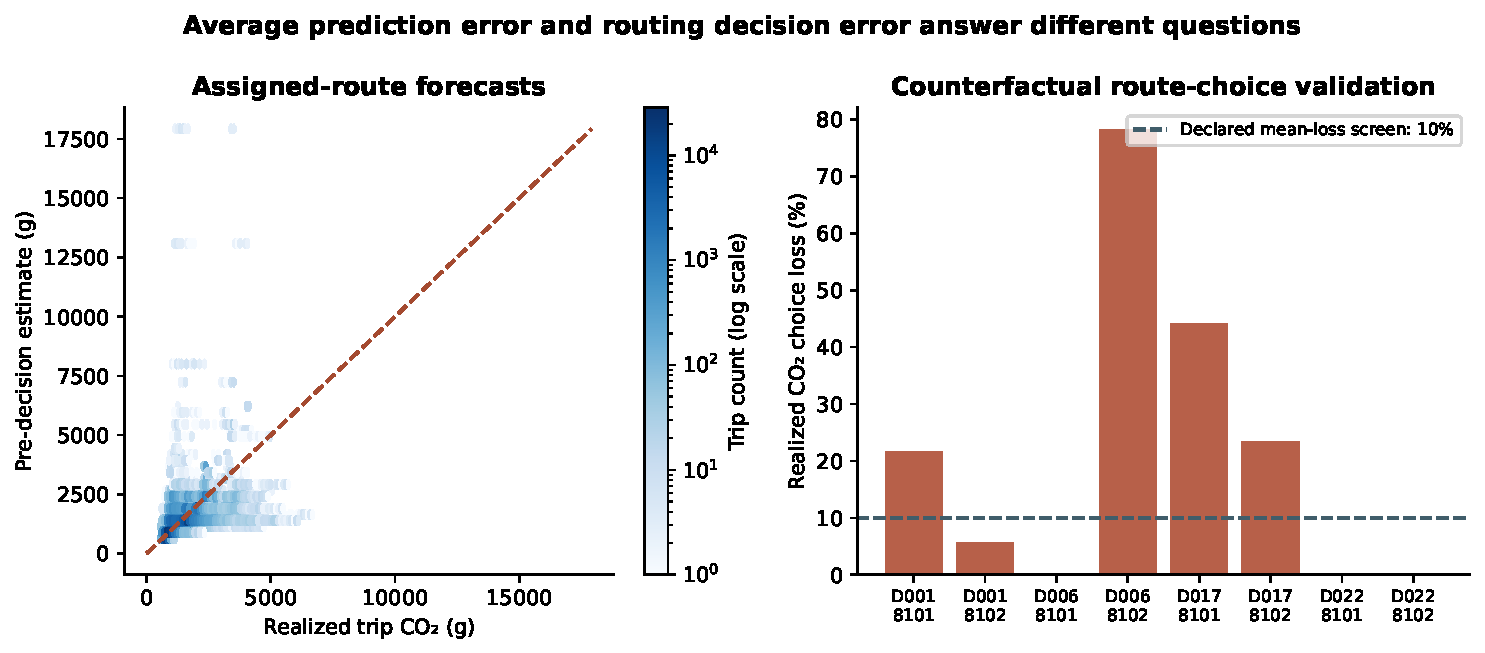
\includegraphics[width=\linewidth]{forecast_and_decision.pdf}
\caption{Aggregate forecast accuracy and marginal route-choice validity are distinct. The right panel covers eight context--seed panels, not 232 independent contexts.}\label{fig:eco}
\end{figure}

\textbf{The preference layer is nearly inert.} Time and \CO\ are strongly aligned in this environment (pooled Spearman 0.982). Repeating the full held-out evaluation at $w_{\text{time}}\in\{0,0.25,0.5,0.75,1\}$ leaves every one of the 24 selector decisions unchanged, and the hindsight-optimal label changes in exactly one context (D011, and only at the pure-emissions extreme). The regime pattern in Section~\ref{sec:regime} is consequently not an artefact of the weights --- it survives the entire admissible weight range --- but it also means the multi-criteria layer here defines preference rather than discriminating between policies. We report this as a property of the environment and decline to present the decision model as a contribution.

\textbf{TECO applies its constraint correctly.} Realised journey time exceeds the $(1+\alpha)$ bound in 54.1\%, 35.6\% and 26.1\% of within-run trips for $\alpha=5,10,15\%$. The constraint is imposed on the \emph{estimated} pre-decision travel time, and these shares compare a realised duration with a predicted benchmark. This is a forecast-to-realised mismatch, not a violation of the algorithm's own constraint. We did not re-audit the implementation source in this study and make no claim beyond the observed shares.

\subsection{Robustness}\label{sec:robust}
\textbf{Hyperparameters.} Across tree depths $\{1,2,3,4,\text{unlimited}\}\times$ leaf sizes $\{1,2,3\}$, headroom capture ranges from 50.9\% to 79.9\% and is positive in all 15 settings. Depth 1 --- a single split on demand --- already captures 53.1\%, confirming that the result rests on regime structure rather than model flexibility.

\textbf{Seeds.} Training on two seed blocks and scoring against the withheld third gives 60.8\%, 67.7\% and 90.2\% capture; the gain is not a replication artefact.

\textbf{Scaling.} Recomputing the evaluation with training-only reference scales rather than common scales gives 79.8\%, so the fold-wise scaling choice does not drive the result.

\textbf{Measurement boundary.} Journey time includes insertion delay while in-network \CO\ excludes pre-insertion idling, and insertion delay is large and strongly policy-dependent at high demand (mean 0.12, 5.54 and 262.41\,s at 720, 1200 and 1680\,veh/h; 810.29\,s in the worst run; 447.5\,s for SP against 6.3\,s for DTT at 1680\,veh/h). Recomputing every decision on in-network time alone changes the preferred policy in \emph{none} of the 24 contexts, and mean headroom only from 0.03018 to 0.03281. The regime structure is therefore not an artefact of the emission accounting boundary, although absolute journey times at high demand clearly are affected by it.

\textbf{Preserved pilot.} An earlier completed 270-run pilot over 30 contexts with SP, DTT and a time-dependent variant gives SP 241.050\,s/639.364\,g, DTT 200.261\,s/506.551\,g and TDR 205.194\,s/523.213\,g, with DTT lowest on both context-average criteria in all 30 contexts and therefore zero adaptive headroom. That environment exhibited no regime reversal; the present network does. The contrast is the reason regime structure must be established empirically before a selector is contemplated.

\section{Discussion}
The practically useful statement is conditional. Adapting the routing policy is worth roughly four fifths of its theoretical value when the deployment regime has been observed during training, and is worse than doing nothing when it has not. For a navigation operator this reframes the engineering question from model selection to instrumentation: the value of policy adaptation is determined by whether the demand and signalisation regimes encountered in service are represented in the data used to fit the selector.

Three points follow. First, a fixed policy is not merely a baseline but the correct choice outside the observed regime span; the safety property of a fixed policy is that its regret cannot be inflated by extrapolation. Second, because the regime boundary is displaced by the signal regime, it is not a property of demand alone, and an operator calibrating such a system would need to cover the signalisation plans in force as well as the demand range. Third, the low model complexity required --- one split on demand recovers half the value --- suggests that effort is better spent on characterising where regimes change than on the selector itself.

The two negative controls are what keep these claims narrow. The environmental objective did not survive contact with a validated route-ordering test, and the preference weights did not change a single decision. A study that reported only the 79.9\% figure, without these, would imply a richer multi-objective problem than this environment contains.

\section{Limitations}
One synthetic topology, one primary OD pair and a homogeneous deterministic fleet are engineered; nothing here is calibrated to a real city and no real-world validation is claimed. Twenty-four contexts and three seed blocks are a small design: leave-one-context-out is the appropriate protocol at this size but is optimistic relative to a single large untouched test set, and no separate confirmatory test set was held back. Demand levels 480\,veh/h apart bracket the reversal without localising it, and the interaction between restriction placement and the crossing point is unresolved. Lane counts are specified rather than calibrated capacities. The environmental estimator is known to be defective for route ordering and its repair was not attempted here. The emission accounting boundary excludes pre-insertion idling. The declared weight profiles are analytical, not elicited from stakeholders. The literature audit was targeted, not systematic, so we assert differences from specific prior studies rather than novelty.

\section{Future work: the minimal localising experiment}\label{sec:future}
The single unresolved quantity is where within each bracket the reversal occurs. Localising it does not require a large factorial. Bisecting the two brackets identified in Table~\ref{tab:margin} requires two additional demand levels --- 960\,veh/h for the balanced bracket and 1440\,veh/h for the arterial bracket --- run over the existing eight restriction/signal cells, three policies and three seeds: 144 additional simulations, roughly 1.5 minutes of compute at the throughput observed for the completed matrix. A second bisection round would halve the remaining interval for a further 144 runs. This experiment characterises the switching regime; it does not increase sample size for the selector, and the selector result above does not depend on it. We specify it here rather than report it: the simulation network, route and configuration files were not available in this session, and running a reconstructed network would have produced results not comparable with the 432 completed runs. No additional simulation was executed and none is reported.

\section{Conclusion}
In a controlled 12-signal urban mesh, the preferred established routing policy reverses with traffic demand --- shortest-distance below the reversal, dynamic travel-time above it --- and the reversal is displaced to higher demand by arterial-priority signal timing. Adapting the policy across this structure is worth 0.03018 mean regret units against the best fixed policy, of which an interpretable depth-3 tree recovers 79.9\% on held-out contexts while being optimal in 21 of 24. Applied outside the demand regimes it was trained on, the same selector is worse than the fixed policy it replaces. Adaptive routing-policy selection is governed by regime coverage of the context space, not by model capacity. An environmental objective and a multi-criteria preference layer were both tested and both found inert in this environment, and are reported as controls rather than removed from the record.

\paragraph{Reproducibility and assistance.}
All reported values derive from the 432 completed runs and the audited project workbook; the analysis scripts regenerate every number in this paper from the exported run table. AI assisted analysis, literature triage and drafting; human authors remain responsible for source verification and submission.

\begin{thebibliography}{45}
\small\setlength{\itemsep}{2pt}\setlength{\parskip}{0pt}
\bibitem{R01} E. W. Dijkstra. A note on two problems in connexion with graphs. Numerische Mathematik, 1959. \url{https://doi.org/10.1007/bf01386390}.
\bibitem{R03} K. Boriboonsomsin; M. J. Barth; W. Zhu; A. Vu. Eco-Routing Navigation System Based on Multisource Historical and Real-Time Traffic Information. IEEE Transactions on Intelligent Transportation Systems, 2012. \url{https://doi.org/10.1109/tits.2012.2204051}.
\bibitem{R04} W. Zeng; T. Miwa; T. Morikawa. Application of the support vector machine and heuristic k-shortest path algorithm to determine the most eco-friendly path with a travel time constraint. Transportation Research Part D, 2017. \url{https://doi.org/10.1016/j.trd.2017.10.001}.
\bibitem{R05} X. Huang; H. Peng. Eco-Routing based on a Data Driven Fuel Consumption Model. arXiv preprint, 2018. \url{https://arxiv.org/abs/1801.08602}.
\bibitem{R08} J. R. Rice. The Algorithm Selection Problem. Advances in Computers 15, 1976. \url{https://doi.org/10.1016/s0065-2458(08)60520-3}.
\bibitem{R09} B. Bischl; P. Kerschke; L. Kotthoff; M. Lindauer; Y. Malitsky; A. Fr\'echette; H. Hoos; F. Hutter; K. Leyton-Brown; K. Tierney; J. Vanschoren. ASlib: A benchmark library for algorithm selection. Artificial Intelligence, 2016. \url{https://doi.org/10.1016/j.artint.2016.04.003}.
\bibitem{R10} L. Xu; F. Hutter; H. H. Hoos; K. Leyton-Brown. SATzilla: Portfolio-based Algorithm Selection for SAT. JAIR, 2008. \url{https://doi.org/10.1613/jair.2490}.
\bibitem{R11} A. N. Elmachtoub; P. Grigas. Smart ``Predict, then Optimize''. Management Science, 2022. \url{https://doi.org/10.1287/mnsc.2020.3922}.
\bibitem{R12} C.-L. Hwang; K. Yoon. Multiple Attribute Decision Making. Springer, 1981. \url{https://doi.org/10.1007/978-3-642-48318-9}.
\bibitem{R13} S. Opricovic; G.-H. Tzeng. Compromise solution by MCDM methods: A comparative analysis of VIKOR and TOPSIS. EJOR 156(2), 2004. \url{https://doi.org/10.1016/S0377-2217(03)00020-1}.
\bibitem{R14} J. P. Brans; Ph. Vincke. Note---A Preference Ranking Organisation Method. Management Science, 1985. \url{https://doi.org/10.1287/mnsc.31.6.647}.
\bibitem{R15} R. L. Keeney; H. Raiffa. Decisions with Multiple Objectives. Cambridge University Press, 1993. \url{https://doi.org/10.1017/cbo9781139174084.005}.
\bibitem{R24} P. Kouvelis; G. Yu. Robust Discrete Optimization and Its Applications. Springer, 1997. \url{https://doi.org/10.1007/978-1-4757-2620-6}.
\bibitem{R37} L. Breiman; J. H. Friedman; R. A. Olshen; C. J. Stone. Classification and Regression Trees. Routledge, 2017. \url{https://doi.org/10.1201/9781315139470}.
\bibitem{R38} X.-F. Xie; Y. Feng; S. F. Smith; K. L. Head. Unified Route Choice Framework: Specification and Application to Urban Traffic Control. Transportation Research Record 2466, 2014. \url{https://doi.org/10.3141/2466-12}.
\bibitem{R40} W. Zeng; T. Miwa; T. Morikawa. Prediction of vehicle CO2 emission and its application to eco-routing navigation. Transportation Research Part C, 2016. \url{https://doi.org/10.1016/j.trc.2016.04.007}.
\bibitem{R41} Routing-induced phase transitions in traffic efficiency of non-Markovian dynamics. Physical Review Research, 2026.
\bibitem{R42} M. A. Falek; A. Gallais; C. Pelsser; S. Julien; F. Theoleyre. To re-route, or not to re-route: Impact of real-time re-routing in urban road networks. Journal of Intelligent Transportation Systems, 2021. \url{https://doi.org/10.1080/15472450.2020.1732205}.
\bibitem{R43} A. Novikov; I. Novikov; A. Katunin. Dynamic traffic re-routing as a method of reducing the congestion level of road network elements. 2018.
\bibitem{R44} J. Chen et al. Efficient detour-aware dynamic routing based on local traffic load in urban road networks. Physical Review E, 2025.
\bibitem{R45} R. Du; S. Chen; Y. Li; J. Dong; P. Y. J. Ha; S. Labi. Dynamic urban traffic rerouting with fog--cloud reinforcement learning. Computer-Aided Civil and Infrastructure Engineering, 2023. \url{https://doi.org/10.1111/mice.12984}.
\end{thebibliography}
\end{document}
